\documentclass[10pt,twocolumn]{article}

\usepackage[margin=0.85in]{geometry}
\usepackage{times}
\usepackage{amsmath}
\usepackage{booktabs}
\usepackage{graphicx}
\usepackage{natbib}
\usepackage{hyperref}
\usepackage{authblk}
\usepackage[T1]{fontenc}

\hypersetup{colorlinks=true, linkcolor=blue, citecolor=blue, urlcolor=blue}

\title{\textbf{Retrieval Succeeds, Reasoning Fails: Disentangling Bottlenecks \\ in Multi-Hop Knowledge Graph Question Answering with Small Language Models}}

\author[1]{Ilahi M. Taofiq\thanks{Corresponding email: taofiqmds24@gmail.com}}
\affil[1]{Independent Research}

\date{}

\begin{document}
\maketitle

\begin{abstract}
Retrieval-augmented generation (RAG) systems are typically evaluated by a single downstream metric: whether the final answer is correct. This conflates two distinct failure modes -- failing to retrieve the right evidence, and failing to reason correctly over evidence that was retrieved -- which require entirely different fixes. We present a controlled study that disentangles these two failure modes for multi-hop question answering. We construct a small synthetic knowledge graph with a fixed relation vocabulary and generate 73 question-answer pairs directly from real graph paths of length 1, 2, and 3 hops, so that every question carries a verifiable gold answer and an exact set of gold supporting facts. We compare three retrieval strategies -- embedding-similarity retrieval (vector RAG), a fixed single-hop graph traversal, and an \emph{agentic} graph traversal that decides for itself, via a small language model's own sufficiency judgment, how many hops to expand -- feeding a 77M-parameter FLAN-T5 model for answer generation. Agentic retrieval achieves the best 2-hop accuracy (74.1\% vs.\ 44.4\% for vector RAG and 0.0\% for fixed single-hop traversal), confirming that adaptive graph traversal helps multi-hop reasoning. At 3 hops, however, agentic retrieval still achieves 93.9\% recall of the gold supporting facts, yet answer accuracy collapses to 9.1\% -- statistically indistinguishable from vector RAG's 9.1\%. This reveals that at this hop depth, the bottleneck is not retrieval but the small model's ability to chain three retrieved facts into a correct answer. We further show that adaptive hop expansion trades retrieval precision for recall, and argue that RAG evaluations for resource-constrained deployments should report retrieval quality and answer accuracy separately, since improving one does not guarantee improving the other.
\end{abstract}

\section{Introduction}

Retrieval-augmented generation \citep{lewis2020rag} is now the default architecture for grounding language model outputs in external facts, and graph-based retrieval -- traversing a knowledge graph rather than searching a vector index -- has been proposed as a way to improve retrieval for questions that require connecting multiple facts \citep{edge2024graphrag}. The implicit assumption behind most RAG evaluations is that better retrieval leads to better answers, and both are usually measured together as a single end-to-end accuracy number.

This conflates two independent failure modes. A RAG pipeline can fail because the retriever did not surface the facts needed to answer the question (a \emph{retrieval failure}), or because the generator was given the correct facts but could not correctly combine them into an answer (a \emph{reasoning failure}). These failures call for different fixes: better retrieval, or a more capable generator. Reporting only final answer accuracy makes it impossible to tell which one is actually responsible for a given error, which matters in particular for teams deploying small, efficient language models under latency or cost constraints, where swapping in a larger generator is not free.

We present a small, fully controlled experiment designed specifically to separate these two failure modes.\footnote{Code, the knowledge graph, the generated question set, and full experimental results are available at \url{https://github.com/taofiq23/GraphRAG-Evidence-Lab}.} We build a synthetic knowledge graph over a closed vocabulary of people, companies, products, and cities, and generate question-answer pairs directly from real paths in the graph using a fixed set of relation-chain templates (Section~\ref{sec:method}). Because every question is generated from an actual graph path, we know its exact gold answer, its exact gold supporting facts, and its true hop count -- ground truth that is difficult to obtain for real-world knowledge graphs but essential for measuring retrieval quality independently of answer correctness.

We compare three retrieval strategies feeding the same small (77M-parameter) FLAN-T5 \citep{chung2022flant5} answer generator: (1) embedding-similarity retrieval over sentence-transformers embeddings \citep{reimers2019sbert} (the standard vector RAG baseline), (2) a fixed single-hop graph traversal, and (3) an \emph{agentic} graph traversal, in the sense used by \citet{yao2023react}, that expands its search radius one hop at a time and asks the generator itself whether the retrieved evidence is sufficient before answering, stopping only when it judges that it is (or a maximum hop count is reached).

Our central finding is that adaptive graph traversal substantially improves 2-hop question answering (Section~\ref{sec:results}), but at 3 hops, retrieval recall remains high (93.9\%) while answer accuracy collapses to the same level as the vector RAG baseline that cannot retrieve the correct facts at all. This is direct evidence that at this hop depth, the bottleneck has moved from retrieval to reasoning -- a distinction invisible to end-to-end accuracy alone.

\textbf{Contributions.} (1) A synthetic knowledge graph and QA generation methodology producing verifiable gold answers and gold supporting facts, enabling retrieval quality and answer accuracy to be measured independently. (2) An empirical comparison of three retrieval strategies, showing that agentic, self-directed graph traversal outperforms both a fixed-hop baseline and vector retrieval at 2 hops. (3) Evidence that at 3 hops, near-perfect retrieval recall does not translate to correct answers with a small generator, isolating a reasoning bottleneck that is distinct from, and not fixed by, improved retrieval. (4) A precision-recall analysis showing that adaptive hop expansion trades retrieval precision for recall as it searches farther from the seed entity.

\section{Related Work}

\textbf{Retrieval-augmented generation.} \citet{lewis2020rag} introduced RAG, combining a parametric generator with a non-parametric retriever over a dense vector index. This architecture is now standard for knowledge-intensive NLP tasks, but treats retrieval as a black box measured only by its effect on final task accuracy.

\textbf{Graph-based retrieval.} \citet{edge2024graphrag} proposed GraphRAG, which builds a knowledge graph from a corpus and retrieves via graph structure rather than embedding similarity, motivated specifically by queries that require synthesizing information spread across a corpus -- the same motivation behind multi-hop question answering. Our work is a small-scale, controlled complement to this line of work: rather than a large corpus-derived graph, we use a synthetic graph with known ground truth specifically to make retrieval quality directly measurable.

\textbf{Multi-hop question answering.} MetaQA \citep{zhang2018metaqa} established multi-hop KGQA as a benchmark task using template-generated questions over a movie-domain knowledge graph, the same general methodology we adopt at a much smaller scale. HotpotQA \citep{yang2018hotpotqa} posed multi-hop questions over free-text Wikipedia passages rather than a structured graph, and additionally required models to identify supporting sentences alongside the answer -- a text-based analogue of the gold-supporting-evidence evaluation we use here. Our contribution is not a new large-scale benchmark but a minimal, fully controlled testbed, with graph-structured ground truth, for isolating retrieval and reasoning failure modes from each other.

\textbf{Adaptive and agentic retrieval.} \citet{yao2023react} introduced ReAct, interleaving reasoning traces with actions (including retrieval) so that a language model can decide what information it needs during generation rather than retrieving once upfront. Our agentic graph traversal strategy applies this idea in a narrower form: the model does not choose retrieval actions freely, but repeatedly judges whether a growing evidence set is sufficient, expanding the graph search radius when it is not.

\textbf{Reasoning in language models.} \citet{wei2022cot} showed that eliciting intermediate reasoning steps (chain-of-thought prompting) improves multi-step reasoning in sufficiently large language models, but this capability is known to be much weaker in small models. Our results are consistent with this: even with all necessary facts retrieved, a 77M-parameter generator does not reliably chain three facts into a correct answer, suggesting that chain-of-thought-style prompting strategies -- and their limits in small models -- are a natural direction for closing the reasoning gap we observe.

\section{Methodology}
\label{sec:method}

\subsection{Knowledge Graph}

We hand-author a knowledge graph of 37 triples over four entity types -- people, companies, products, and cities -- and six relation types: \texttt{founded}, \texttt{ceo\_of}, \texttt{based\_in}, \texttt{created}, \texttt{works\_at}, and \texttt{acquired\_by}. Founder and CEO are deliberately different people at every company: an early iteration of this graph made founder and CEO the same person, which caused a structural ambiguity in an earlier, since-abandoned stopping heuristic for the agentic retriever (Section~\ref{sec:agentic}) that we discuss in Appendix~\ref{sec:appendix-design}. The \texttt{works\_at} relation is included as intentional distractor data, present in the graph but never targeted by any question template, to test whether retrieval methods pull in irrelevant facts.

\subsection{Question Generation}

Questions are generated programmatically from six single-hop relation-chain patterns and their compositions into 2-hop and 3-hop chains (e.g., ``Who founded the company that created \emph{X}?'' composes a \texttt{created} edge with a \texttt{founded} edge). Because each question is instantiated from a real path that actually exists in the graph, every example carries: (a) a gold answer, (b) the exact ordered list of gold supporting triples along that path, and (c) a ground-truth hop count. This yields 73 questions: 35 one-hop, 27 two-hop, and 11 three-hop. Only one entity is named explicitly in the question text for 2- and 3-hop questions (e.g., only the product name in ``Who founded the company that created \emph{X}?''); the rest of the answer chain must be discovered through retrieval, which is what makes multi-hop retrieval nontrivial in this setup.

\subsection{Retrieval Strategies}

\textbf{Vector RAG.} Every triple in the graph is rendered as a natural-language sentence (e.g., ``Alice founded Nova Tech.'') and embedded with \texttt{all-MiniLM-L6-v2} \citep{reimers2019sbert}. At query time, the top-3 sentences by cosine similarity to the question are retrieved.

\textbf{Fixed 1-hop GraphRAG.} The entity named in the question is identified via exact string matching against the graph's vocabulary, and its full 1-hop neighborhood (all triples touching that entity) is retrieved.

\label{sec:agentic}
\textbf{Agentic GraphRAG.} Retrieval begins at the named entity's 1-hop neighborhood. The generator is then prompted to judge, in natural language, whether the retrieved context is sufficient to answer the question. If it judges the context insufficient, the search radius expands to 2 hops and the question is asked again, up to a maximum of 3 hops. This is a genuinely adaptive procedure: the number of hops used is decided by the model at inference time, not fixed in advance or derived from the question's true hop count.

\subsection{Answer Generation and Evaluation}

All three strategies feed their retrieved evidence, rendered as natural-language sentences, to the same \texttt{google/flan-t5-small} model (77M parameters), prompted to answer using only the given context. We report:

\begin{itemize}
    \item \textbf{Answer accuracy}: whether the gold answer string appears in the generated answer (case-insensitive containment), the standard lenient metric for evaluating short-form generative QA with small models.
    \item \textbf{Retrieval precision/recall}: computed by treating each system's retrieved set of triples as a set and comparing it against the gold supporting triples for that question.
\end{itemize}

\subsection{Implementation Details and Reproducibility}
\label{sec:implementation}

The knowledge graph and question set are generated with a fixed random seed (0), so the exact 73-question evaluation set used throughout this paper is deterministic and reproducible from the released code. Vector RAG retrieves the top $k{=}3$ sentences by cosine similarity. Agentic GraphRAG expands to a maximum of 3 hops, matching the maximum ground-truth hop count in the question set; at each hop it issues one sufficiency-judgment prompt and, if satisfied, one answer-generation prompt to \texttt{flan-t5-small}, both using greedy decoding (no sampling) for determinism. All retrieved evidence is rendered as natural-language sentences via fixed templates (e.g., \texttt{(subject, founded, object)} $\rightarrow$ ``Subject founded Object.'') before being passed to the generator, so every system sees evidence in the same textual format and differences in accuracy reflect \emph{which} facts were retrieved, not how they were phrased. All experiments run on CPU; no GPU or model training is required to reproduce any result in this paper.

\section{Results}
\label{sec:results}

Table~\ref{tab:accuracy} reports answer accuracy by ground-truth hop count, and Figure~\ref{fig:accuracy} visualizes the same data. Table~\ref{tab:retrieval} reports retrieval precision and recall for the same configurations.

\begin{table}[t]
\centering
\small
\begin{tabular}{lccc}
\toprule
\textbf{System} & \textbf{1-hop} & \textbf{2-hop} & \textbf{3-hop} \\
& (n=35) & (n=27) & (n=11) \\
\midrule
Vector RAG            & 100.0\% & 44.4\% & 9.1\% \\
Fixed 1-hop GraphRAG   & 100.0\% & 0.0\%  & 0.0\% \\
Agentic GraphRAG       & 100.0\% & \textbf{74.1\%} & 9.1\% \\
\bottomrule
\end{tabular}
\caption{Answer accuracy by ground-truth hop count.}
\label{tab:accuracy}
\end{table}

\begin{figure}[t]
\centering
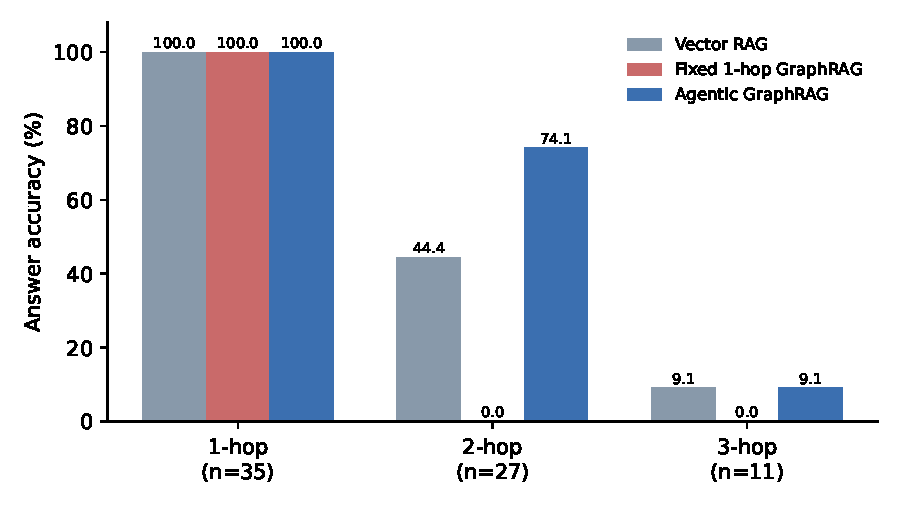
\includegraphics[width=\linewidth]{accuracy_by_hop.pdf}
\caption{Answer accuracy by ground-truth hop count (same data as Table~\ref{tab:accuracy}). Agentic GraphRAG's advantage is concentrated entirely at 2 hops; all three systems converge at 1 and 3 hops, for different reasons (Section~\ref{sec:results}).}
\label{fig:accuracy}
\end{figure}

\begin{table}[t]
\centering
\small
\begin{tabular}{lccc}
\toprule
\textbf{System} & \textbf{1-hop} & \textbf{2-hop} & \textbf{3-hop} \\
\midrule
\multicolumn{4}{l}{\textit{Retrieval precision}} \\
Vector RAG            & 33.3\% & 46.9\% & 36.4\% \\
Fixed 1-hop GraphRAG   & 31.1\% & 51.9\% & 63.6\% \\
Agentic GraphRAG       & 27.8\% & 17.4\% & 24.9\% \\
\midrule
\multicolumn{4}{l}{\textit{Retrieval recall}} \\
Vector RAG            & 100.0\% & 70.4\% & 36.4\% \\
Fixed 1-hop GraphRAG   & 100.0\% & 50.0\% & 33.3\% \\
Agentic GraphRAG       & 100.0\% & 100.0\% & \textbf{93.9\%} \\
\midrule
\multicolumn{4}{l}{\textit{Avg.\ hops used (agentic only)}} \\
Agentic GraphRAG       & 1.43 & 2.89 & 2.82 \\
\bottomrule
\end{tabular}
\caption{Retrieval precision and recall against gold supporting triples, and the agentic system's average hop count, by ground-truth hop count.}
\label{tab:retrieval}
\end{table}

\textbf{1-hop questions are solved by every system.} A single relevant fact is easy for embedding similarity to surface, leaving no room for graph traversal to add value.

\textbf{At 2 hops, agentic graph traversal wins decisively.} Fixed 1-hop retrieval is structurally incapable of reaching the second fact in the chain, and scores 0\% -- not a modeling failure but a direct consequence of the retrieval radius being too small by design. Vector RAG partially succeeds (44.4\%) when one of the two required facts happens to be lexically similar to the question. Agentic retrieval reaches 100\% recall by adaptively expanding its search (using an average of 2.89 hops for ground-truth 2-hop questions) and converts that into 74.1\% answer accuracy.

\textbf{At 3 hops, retrieval and reasoning diverge.} Agentic retrieval still achieves 93.9\% recall -- it is finding the facts it needs almost every time, using an average of 2.82 hops. Yet answer accuracy is 9.1\%, statistically indistinguishable from vector RAG's 9.1\% (both are 1 correct answer out of 11 questions; we caution against reading much into the exact match at this small sample size, but the qualitative point -- that accuracy did not track the much higher recall -- is robust). Handing the generator all three correct facts is not sufficient for it to chain them into the right final answer.

\textbf{Adaptive expansion trades precision for recall.} Agentic retrieval's precision falls from 27.8\% (1-hop) to 17.4\% (2-hop) as its search radius grows, since a wider graph neighborhood pulls in real but irrelevant facts (a company's other products, an unrelated employee) alongside the ones actually needed. This is a genuine cost of recall-maximizing retrieval that a deployment relying on retrieved-context length or downstream re-ranking would need to account for.

\section{Qualitative Error Analysis}
\label{sec:qualitative}

Aggregate metrics show \emph{that} accuracy diverges from recall; inspecting individual outputs shows one concrete way this happens. Consider the 2-hop question ``Which company acquired the company founded by Heidi?'' (gold answer: \emph{Solstice Robotics}; gold supporting facts: \emph{Heidi founded Pixel Forge} and \emph{Pixel Forge was acquired by Solstice Robotics}).

Agentic GraphRAG's retrieved evidence for this question included both gold facts verbatim, alongside eight other true-but-irrelevant facts about Pixel Forge and Solstice Robotics pulled in by the 2-hop neighborhood expansion (e.g., their locations, other products, other employees) -- a concrete instance of the precision cost described in Section~\ref{sec:results}. Despite the correct evidence being present, the generated answer was \emph{``Pixel Forge''}: the object of the \texttt{founded} relation named in the question, not the object of the \texttt{acquired\_by} relation actually being asked about. Vector RAG, with a much smaller and different retrieved set, produced the identical wrong answer, \emph{``Pixel Forge.''}

We read this as evidence of a relation-identification failure rather than a retrieval failure: the generator appears to default to an entity that is lexically prominent in the combined question-and-context text (Pixel Forge is named in the question itself and appears in nearly every retrieved sentence) rather than correctly tracing which relation edge the question asks about. This is consistent with the aggregate 3-hop collapse in Section~\ref{sec:results} and suggests that the failure is not idiosyncratic to long chains specifically, but to any case where the correct answer requires distinguishing the \emph{target} of a specific relation from other entities that are simply present and salient in the context.

\section{Discussion}

The central implication of Table~\ref{tab:accuracy} and Table~\ref{tab:retrieval} together is that \emph{retrieval quality and answer accuracy are separate axes that can move independently}, and a system evaluated only on the latter would misdiagnose the 3-hop failure. Someone observing only the 9.1\% accuracy number might reasonably conclude the retriever needs improvement; the recall numbers show that would be the wrong fix, since retrieval was already finding 93.9\% of the needed facts. The correct fix in this case is a more capable generator, better reasoning prompting (e.g., chain-of-thought), or explicit multi-step answer composition -- not further retrieval engineering.

This matters most for exactly the deployment setting a small 77M-parameter generator represents: teams choosing an efficient model for cost or latency reasons need to know whether their retrieval investment is actually being converted into better answers, or whether they have hit a reasoning ceiling that no amount of additional retrieval engineering will lift. We suggest that RAG evaluations, particularly in resource-constrained settings, report retrieval-quality metrics (precision/recall against known relevant evidence, where available) alongside end-to-end accuracy, rather than accuracy alone.

\section{Limitations}

Our knowledge graph is small (37 triples) and synthetic, built specifically to provide verifiable gold answers and supporting facts -- a necessary trade-off for isolating retrieval from reasoning failures, but one that does not speak to retrieval quality on large, noisy, real-world corpora. The 3-hop condition has only 11 questions, and while the qualitative retrieval-recall-versus-accuracy divergence is clear, exact accuracy percentages at this sample size carry wide uncertainty. Answer correctness is judged by lenient string containment, standard for evaluating small generative models but coarser than exact-match or human evaluation. We study a single small generator (FLAN-T5-small); whether the reasoning bottleneck we observe persists, narrows, or disappears with larger models is an open question we did not test and consider the most direct follow-up to this work. Finally, our agentic stopping criterion is itself an unverified LLM self-judgment with no ground truth backing it -- its own reliability, which our results suggest is imperfect at higher hop counts, is part of what this study surfaces rather than an assumption it depends on.

\section{Ethics Statement}

This work uses an entirely synthetic, hand-authored knowledge graph and programmatically generated questions. It does not involve human subjects, crowdsourced annotation, personally identifiable information, or web-scraped content, and we do not foresee direct ethical concerns arising from it. We note the broader concern, applicable to any RAG evaluation, that a system with high retrieval recall but low answer accuracy (Section~\ref{sec:results}) could appear well-grounded in evidence while still producing incorrect answers -- exactly the situation where a lenient end-to-end accuracy metric could mislead a deployment decision if retrieval-quality metrics are not reported alongside it, which is the practice this paper argues for.

\section{Conclusion}

We presented a controlled study isolating retrieval quality from answer accuracy in multi-hop knowledge graph question answering. Agentic, self-directed graph traversal substantially outperforms both vector retrieval and fixed-hop graph traversal at 2-hop questions, confirming the value of adaptive retrieval depth. At 3 hops, however, near-perfect retrieval recall (93.9\%) does not prevent a collapse in answer accuracy (9.1\%), demonstrating that retrieval and reasoning are separable failure modes that end-to-end accuracy alone cannot distinguish. We release our knowledge graph, question generation code, and full experimental pipeline to support further controlled studies of this kind.

\bibliographystyle{plainnat}
\begin{thebibliography}{9}

\bibitem[Chung et al.(2022)]{chung2022flant5}
Hyung Won Chung, Le Hou, Shayne Longpre, et al.
\newblock Scaling Instruction-Finetuned Language Models.
\newblock \emph{arXiv preprint}, 2022.

\bibitem[Edge et al.(2024)]{edge2024graphrag}
Darren Edge, Ha Trinh, Newman Cheng, et al.
\newblock From Local to Global: A Graph RAG Approach to Query-Focused Summarization.
\newblock \emph{arXiv preprint}, 2024.

\bibitem[Lewis et al.(2020)]{lewis2020rag}
Patrick Lewis, Ethan Perez, Aleksandra Piktus, et al.
\newblock Retrieval-Augmented Generation for Knowledge-Intensive NLP Tasks.
\newblock \emph{Advances in Neural Information Processing Systems (NeurIPS)}, 2020.

\bibitem[Reimers and Gurevych(2019)]{reimers2019sbert}
Nils Reimers and Iryna Gurevych.
\newblock Sentence-BERT: Sentence Embeddings using Siamese BERT-Networks.
\newblock \emph{Proceedings of EMNLP-IJCNLP}, 2019.

\bibitem[Wei et al.(2022)]{wei2022cot}
Jason Wei, Xuezhi Wang, Dale Schuurmans, et al.
\newblock Chain-of-Thought Prompting Elicits Reasoning in Large Language Models.
\newblock \emph{Advances in Neural Information Processing Systems (NeurIPS)}, 2022.

\bibitem[Yang et al.(2018)]{yang2018hotpotqa}
Zhilin Yang, Peng Qi, Saizheng Zhang, et al.
\newblock HotpotQA: A Dataset for Diverse, Explainable Multi-hop Question Answering.
\newblock \emph{Proceedings of EMNLP}, 2018.

\bibitem[Yao et al.(2023)]{yao2023react}
Shunyu Yao, Jeffrey Zhao, Dian Yu, et al.
\newblock ReAct: Synergizing Reasoning and Acting in Language Models.
\newblock \emph{International Conference on Learning Representations (ICLR)}, 2023.

\bibitem[Zhang et al.(2018)]{zhang2018metaqa}
Yuyu Zhang, Hanjun Dai, Zornitsa Kozareva, et al.
\newblock Variational Reasoning for Question Answering with Knowledge Graph.
\newblock \emph{Proceedings of AAAI}, 2018.

\end{thebibliography}

\appendix
\section{Design Note: An Abandoned Stopping Heuristic}
\label{sec:appendix-design}

An earlier iteration of the agentic retriever used a structural stopping rule instead of LLM self-judgment: expand hops until the retrieved subgraph contains a fact whose relation type matches the question's expected answer type (e.g., a \texttt{ceo\_of} fact for a ``who is the CEO'' question). This failed for chains like ``who is the CEO of the company that acquired the company that created \emph{X}'', because the \emph{intermediate} company in the chain also has its own CEO, reachable one hop earlier than the true target company's CEO -- the heuristic matched the wrong fact and stopped early. This failure mode does not depend on the founder/CEO identity ambiguity described in Section~\ref{sec:method}, but is worth recording as a cautionary example of why type-matching alone is an unreliable retrieval-sufficiency signal, which motivated the switch to LLM self-judgment reported in the main text.

\end{document}
